%
% File coling2020.tex
%
% Contact: feiliu@cs.ucf.edu & liang.huang.sh@gmail.com
%% Based on the style files for COLING-2018, which were, in turn,
%% Based on the style files for COLING-2016, which were, in turn,
%% Based on the style files for COLING-2014, which were, in turn,
%% Based on the style files for ACL-2014, which were, in turn,
%% Based on the style files for ACL-2013, which were, in turn,
%% Based on the style files for ACL-2012, which were, in turn,
%% based on the style files for ACL-2011, which were, in turn, 
%% based on the style files for ACL-2010, which were, in turn, 
%% based on the style files for ACL-IJCNLP-2009, which were, in turn,
%% based on the style files for EACL-2009 and IJCNLP-2008...

%% Based on the style files for EACL 2006 by 
%%e.agirre@ehu.es or Sergi.Balari@uab.es
%% and that of ACL 08 by Joakim Nivre and Noah Smith

\documentclass[11pt]{article}
\usepackage{coling2020}
\usepackage{times}
\usepackage{url}
\usepackage{latexsym}
\usepackage{indentfirst}

\usepackage{times}
\usepackage{latexsym}
\usepackage{times}
\usepackage{soul}
\usepackage{url}
\usepackage{amsmath}
\usepackage{amsthm}
\usepackage{booktabs}
\usepackage{algorithm}
\usepackage{algorithmic}
\usepackage{amssymb}
\usepackage{longtable}
\usepackage{graphicx}
\usepackage{CJK}
\usepackage{multirow}
\usepackage{color}

%\setlength\titlebox{5cm}
\colingfinalcopy % Uncomment this line for the final submission

% You can expand the titlebox if you need extra space
% to show all the authors. Please do not make the titlebox
% smaller than 5cm (the original size); we will check this
% in the camera-ready version and ask you to change it back.


\title{2021年04月13日进度汇报}

\author{屈原斌 \\
  首都师范大学 \\
    {\tt ybqu@cnu.edu.cn}}

\date{}

\begin{document}
\begin{CJK}{UTF8}{gkai}

\maketitle
\CJKindent
%\begin{abstract}

%\end{abstract}

\section{今日进度}


\begin{itemize}
  \item [1.] 英文离题指标更新
  \item [2.] 标题-正文匹配数据check
  \item [3.] 成语古诗文检错方案指标更新
\end{itemize}

\section{工作详述}
\subsection{英文离题指标更新}
\subsubsection{微调生成模型}
\begin{itemize}
  \item 数据:1931篇英语作文数据
\end{itemize}

\subsubsection{离题指标更新}
\begin{itemize}
  \item 数据:ICLE英文数据集,按照[2.0,2.5,3.0]和[3.5,4.0]划分离题和切题数据,数据比例:离题:切题=157:673(1:4.3)
  \item 实验方案:(五折交叉验证)(生成模型和SVC结果未整理出来)
  \begin{itemize}
    \item 方案一:基于题目排序方案,实验结果见表1、3
    \item 方案二:基于相似度方案,实验结果见表2、4
    \item 方案三:基于特征的SVC,实验结果见表5
  \end{itemize}
\end{itemize}

% Table generated by Excel2LaTeX from sheet '3.0划分(Accuracy)'
\begin{table}[htbp]\small
  \centering
  \begin{tabular}{cc|ccccccc}
    \hline
    \multicolumn{2}{c}{\multirow{2}[0]{*}{\textcolor[rgb]{ 1,  0,  0}{}}} & \multirow{2}[0]{*}{\textbf{Accuracy}} & \multicolumn{3}{c}{\textbf{离题}} & \multicolumn{3}{c}{\textbf{不离题}} \\
    \multicolumn{2}{c}{} &       & \textbf{precision} & \textbf{recall} & \textbf{f1-score} & \textbf{precision} & \textbf{recall} & \textbf{f1-score} \\
    \hline
    \multirow{2}[0]{*}{doc2vec} & 开发集   & 0.9386  & 0.2000  & 0.0182  & 0.0333  & 0.9385  & 1.0000  & 0.9682  \\
    & 验证集   & 0.9334  & 0.3452  & 0.0192  & 0.0352  & 0.9382  & 0.9945  & 0.9655  \\
    \hline
    \multirow{2}[0]{*}{habilstm} & 开发集   & 0.9422  & 0.7000  & 0.1060  & 0.1794  & 0.9440  & 0.9974  & 0.9699  \\
    & 验证集   & 0.9364  & 0.5558  & 0.0920  & 0.1525  & 0.9424  & 0.9929  & 0.9670  \\
    \hline
    \multirow{2}[0]{*}{bert} & 开发集   & 0.9446  & 0.7200  & 0.1421  & 0.2299  & 0.9463  & 0.9974  & 0.9711  \\
    & 验证集   & 0.9301  & 0.4914  & 0.0870  & 0.1282  & 0.9418  & 0.9865  & 0.9636  \\
    \hline
    \multirow{2}[0]{*}{bert\_whitening} & 开发集   & 0.8602  & 0.0375  & 0.0321  & 0.0333  & 0.9345  & 0.9154  & 0.9246  \\
    & 验证集   & 0.8602  & 0.0297  & 0.0381  & 0.0333  & 0.9344  & 0.9152  & 0.9247  \\
    \hline
    \multirow{2}[0]{*}{bertabs} & 开发集   &       &       &       &       &       &       &  \\
    & 验证集   &       &       &       &       &       &       &  \\
    \hline
  \end{tabular}%
  \caption{方案一实验结果(Accuracy调阈值)}
  \label{tab:addlabel}%
\end{table}%


% Table generated by Excel2LaTeX from sheet '3.0划分(Accuracy)'
\begin{table}[htbp]\small
  \centering
  \begin{tabular}{cc|ccccccc}
    \hline
    \multicolumn{2}{c}{\multirow{2}[1]{*}{\textcolor[rgb]{ 1,  0,  0}{}}} & \multirow{2}[1]{*}{\textbf{Accuracy}} & \multicolumn{3}{c}{\textbf{离题}} & \multicolumn{3}{c|}{\textbf{不离题}} \\
    \multicolumn{2}{c}{} &       & \textbf{precision} & \textbf{recall} & \textbf{f1-score} & \textbf{precision} & \textbf{recall} & \multicolumn{1}{c}{\textbf{f1-score}} \\
    \hline
    \multirow{2}[0]{*}{doc2vec} & 开发集   & 0.9446  & 0.6000  & 0.0964  & 0.1582  & 0.9442  & 1.0000  & 0.9713  \\
    & 验证集   & 0.9373  & 0.3000  & 0.0253  & 0.0455  & 0.9387  & 0.9984  & 0.9676  \\
    \hline
    \multirow{2}[0]{*}{habilstm} & 开发集   & 0.9410  & 0.7000  & 0.1060  & 0.1794  & 0.9439  & 0.9961  & 0.9693  \\
    & 验证集   & 0.9377  & 0.5133  & 0.0770  & 0.1334  & 0.9416  & 0.9952  & 0.9677  \\
    \hline
    \multirow{2}[0]{*}{bert} & 开发集   & 0.9422  & 0.6167  & 0.1199  & 0.1963  & 0.9451  & 0.9961  & 0.9699  \\
    & 验证集   & 0.9337  & 0.5328  & 0.0775  & 0.1202  & 0.9414  & 0.9910  & 0.9655  \\
    \hline
    \multirow{2}[0]{*}{bert\_whitening} & 开发集   & 0.1289  & 0.0639  & 0.9262  & 0.1192  & 0.9470  & 0.0747  & 0.1381  \\
    & 验证集   & 0.1289  & 0.0637  & 0.9416  & 0.1194  & 0.9504  & 0.0746  & 0.1383  \\
    \hline
    \multirow{2}[0]{*}{bertabs} & 开发集   &       &       &       &       &       &       &  \\
    & 验证集   &       &       &       &       &       &       &  \\
    \hline
        \end{tabular}%
        \caption{方案二实验结果(Accuracy调阈值)}
  \label{tab:addlabel}%
\end{table}%


% Table generated by Excel2LaTeX from sheet '3.0划分(F1-score调阈值)'
\begin{table}[htbp]\small
  \centering
  \begin{tabular}{cc|ccccccc}
    \hline
    \multicolumn{2}{c}{\multirow{2}[0]{*}{\textcolor[rgb]{ 1,  0,  0}{}}} & \multirow{2}[0]{*}{\textbf{Accuracy}} & \multicolumn{3}{c}{\textbf{离题}} & \multicolumn{3}{c}{\textbf{不离题}} \\
    \multicolumn{2}{c}{} &       & \textbf{precision} & \textbf{recall} & \textbf{f1-score} & \textbf{precision} & \textbf{recall} & \textbf{f1-score} \\
    \hline
    \multirow{2}[0]{*}{doc2vec} & 开发集   & 0.8639  & 0.3269  & 0.1874  & 0.1657  & 0.9441  & 0.9091  & 0.9247  \\
    & 验证集   & 0.8506  & 0.0751  & 0.1471  & 0.0938  & 0.9405  & 0.8974  & 0.9169  \\
    \hline
    \multirow{2}[0]{*}{habilstm} & 开发集   & 0.9205  & 0.4412  & 0.2351  & 0.2643  & 0.9506  & 0.9652  & 0.9578  \\
    & 验证集   & 0.9072  & 0.2887  & 0.2027  & 0.2097  & 0.9472  & 0.9544  & 0.9506  \\
    \hline
    \multirow{2}[0]{*}{bert} & 开发集   & 0.8253  & 0.5615  & 0.2746  & 0.2466  & 0.9463  & 0.8662  & 0.8839  \\
    & 验证集   & 0.8259  & 0.2571  & 0.2452  & 0.1619  & 0.9466  & 0.8635  & 0.8824  \\
    \hline
    \multirow{2}[0]{*}{bert\_whitening} & 开发集   & 0.5602  & 0.0835  & 0.4462  & 0.1285  & 0.9355  & 0.5694  & 0.6826  \\
    & 验证集   & 0.5470  & 0.0486  & 0.3519  & 0.0836  & 0.9260  & 0.5596  & 0.6756  \\
    \hline
    \multirow{2}[0]{*}{bertabs} & 开发集   &       &       &       &       &       &       &  \\
    & 验证集   &       &       &       &       &       &       &  \\
    \hline
        \end{tabular}%
        \caption{方案一实验结果(F1-score调阈值)}
  \label{tab:addlabel}%
\end{table}%

% Table generated by Excel2LaTeX from sheet '3.0划分(F1-score调阈值)'
\begin{table}[htbp]\small
  \centering
  \begin{tabular}{cc|ccccccc}
    \hline
    \multicolumn{2}{c}{\multirow{2}[0]{*}{\textcolor[rgb]{ 1,  0,  0}{}}} & \multirow{2}[0]{*}{\textbf{Accuracy}} & \multicolumn{3}{c}{\textbf{离题}} & \multicolumn{3}{c}{\textbf{不离题}} \\
    \multicolumn{2}{c}{} &       & \textbf{precision} & \textbf{recall} & \textbf{f1-score} & \textbf{precision} & \textbf{recall} & \textbf{f1-score} \\
    \hline
    \multirow{2}[0]{*}{doc2vec} & 开发集   & 0.8157  & 0.3239  & 0.3859  & 0.2602  & 0.9535  & 0.8476  & 0.8879  \\
    & 验证集   & 0.8190  & 0.2424  & 0.3760  & 0.2190  & 0.9544  & 0.8475  & 0.8879  \\
    \hline
    \multirow{2}[0]{*}{habilstm} & 开发集   & 0.9024  & 0.2694  & 0.2949  & 0.2734  & 0.9532  & 0.9422  & 0.9474  \\
    & 验证集   & 0.8952  & 0.2124  & 0.2213  & 0.2053  & 0.9476  & 0.9402  & 0.9436  \\
    \hline
    \multirow{2}[0]{*}{bert} & 开发集   & 0.7482  & 0.4699  & 0.4792  & 0.2816  & 0.9619  & 0.7720  & 0.8027  \\
    & 验证集   & 0.7364  & 0.1802  & 0.3155  & 0.1280  & 0.9446  & 0.7630  & 0.7962  \\
    \hline
    \multirow{2}[0]{*}{bert\_whitening} & 开发集   & 0.1108  & 0.0662  & 1.0000  & 0.1237  & 0.8000  & 0.0517  & 0.0954  \\
    & 验证集   & 0.1057  & 0.0630  & 0.9560  & 0.1181  & 0.9626  & 0.0488  & 0.0912  \\
    \hline
    \multirow{2}[0]{*}{bertabs} & 开发集   &       &       &       &       &       &       &  \\
    & 验证集   &       &       &       &       &       &       &  \\
    \hline
  \end{tabular}%
  \caption{方案二实验结果(F1-score调阈值)}
  \label{tab:addlabel}%
\end{table}%


% Table generated by Excel2LaTeX from sheet '中文数据集'
% \begin{figure*}[htbp]\small
%   \centering
%   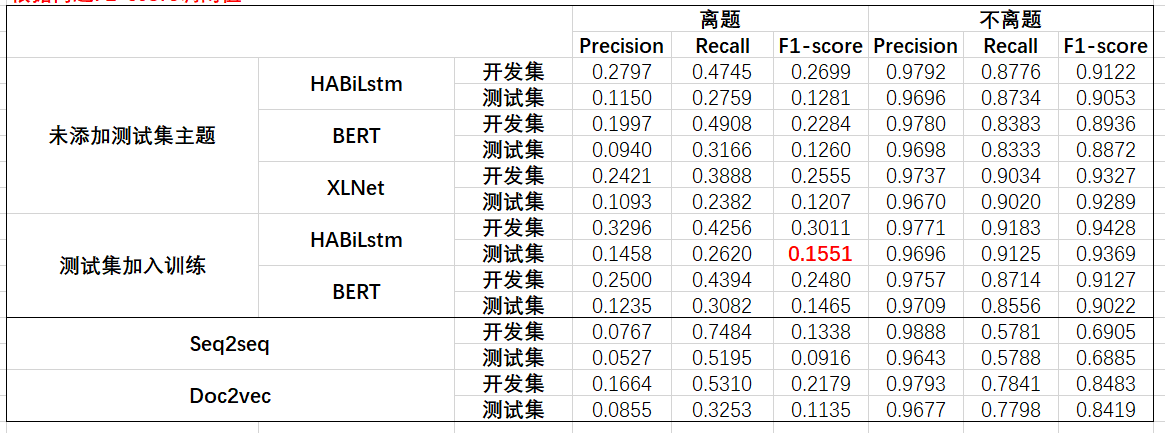
\includegraphics[width=1.0\linewidth]{zb.png}
%   \caption{生成样例2}
%   \label{framework}
% \end{figure*}

%\bibliography{reference}
%\bibliographystyle{coling}
%\bibliography{coling2020}

\end{CJK}
\end{document}


% include your own bib file like this:


%\begin{thebibliography}{}

%\bibitem[\protect\citename{Aho and Ullman}1972]{Aho:72}
%Alfred~V. Aho and Jeffrey~D. Ullman.
%\newblock 1972.
%\newblock {\em The Theory of Parsing, Translation and Compiling}, volume~1.
%\newblock Prentice-{Hall}, Englewood Cliffs, NJ.

%\bibitem[\protect\citename{{American Psychological Association}}1983]{APA:83}
%{American Psychological Association}.
%\newblock 1983.
%\newblock {\em Publications Manual}.
%\newblock American Psychological Association, Washington, DC.

%\bibitem[\protect\citename{{Association for Computing Machinery}}1983]{ACM:83}
%{Association for Computing Machinery}.
%\newblock 1983.
%\newblock {\em Computing Reviews}, 24(11):503--512.

%\bibitem[\protect\citename{Chandra \bgroup et al.\egroup }1981]{Chandra:81}
%Ashok~K. Chandra, Dexter~C. Kozen, and Larry~J. Stockmeyer.
%\newblock 1981.
%\newblock Alternation.
%\newblock {\em Journal of the Association for Computing Machinery},
%  28(1):114--133.

%\bibitem[\protect\citename{Gusfield}1997]{Gusfield:97}
%Dan Gusfield.
%\newblock 1997.
%\newblock {\em Algorithms on Strings, Trees and Sequences}.
%\newblock Cambridge University Press, Cambridge, UK.

%\bibitem[\protect\citename{Rasooli and Tetreault}2015]{rasooli-tetrault-2015}
%Mohammad~Sadegh Rasooli and Joel~R. Tetreault. 2015.
%\newblock {Yara parser: {A} fast and accurate dependency parser}.
%\newblock \emph{Computing Research Repository}, arXiv:1503.06733.
%\newblock Version 2.

%\bibitem[\protect\citename{Borschinger and Johnson}2011]{borsch2011}
%Benjamin Borschinger and Mark Johnson. 2011.
%\newblock A particle filter algorithm for {B}ayesian wordsegmentation.
%\newblock In \emph{Proceedings of the Australasian Language Technology Association %Workshop 2011}, pages 10--18, Canberra, Australia.

%\end{thebibliography}

